\documentclass[a4paper,11pt]{proc}
\usepackage[a4paper,margin=2cm,footskip=1cm]{geometry}
\usepackage[utf8]{inputenc}
\usepackage{fancyhdr}
\usepackage{graphicx}
\usepackage{listings}
\usepackage{xcolor}
\usepackage{textcomp}
\usepackage[section]{placeins}
\usepackage[T1]{fontenc}

\definecolor{codegreen}{rgb}{0,0.6,0}
\definecolor{codegray}{rgb}{0.5,0.5,0.5}
\definecolor{codepurple}{rgb}{0.58,0,0.82}
\definecolor{backcolour}{rgb}{0.95,0.95,0.92}
\definecolor{codepurple}{HTML}{C42043}
\definecolor{backcolour}{HTML}{F2F2F2}
\definecolor{bookColor}{cmyk}{0,0,0,0.90}  
\color{bookColor}

\lstset{upquote=true}

\lstdefinestyle{mystyle}{
	backgroundcolor=\color{backcolour},   
	commentstyle=\color{codegreen},
	keywordstyle=\color{codepurple},
	numberstyle=\footnotesize\color{codegray},
	stringstyle=\color{codepurple},
	basicstyle=\footnotesize,
	breakatwhitespace=false,         
	breaklines=true,                 
	captionpos=b,                    
	keepspaces=true,                 
	numbers=left,                    
	numbersep=10pt,                  
	showspaces=false,                
	showstringspaces=false,
	showtabs=false,      
}
\lstset{style=mystyle} 

\pagestyle{fancy}
\title{Prawn King Documentation}
\author{Rohan Chikkam}

\rhead{Prawn King Documentation}
\lhead{Reading School - 51337}
\rfoot{Rohan Chikkam - 9051}

\begin{document}

\begin{titlepage}

\maketitle
\end{titlepage}

\section{Introduction}

    \begin{itemize}
      \item Agricultural Practice in Greater India
      \item Aquatic Agricultural Practice
    \end{itemize}

\section{Analysis}

    \begin{itemize}
      \item Traditional Data Collection Methods
      \item Real World Problem
      \item Pre-development: Client Interviews
      \item Pre-development: Questionnaires
      \item Viable Solutions
    \end{itemize}

\section{Design}

    \begin{itemize}
      \item The Solution
      \item Data Flow Model
      \item Project Pipeline
    \end{itemize}

\section{Implementation}
    
    \begin{itemize}
      \item Overview1234
      \item Data Collection and Improvement
    \end{itemize}

\section{Testing}

    \begin{itemize}
      \item Algorithmic Testing
      \item Reliability Testing
      \item Security / Data Integrity Testing
      \item Post-development: Client Interviews
      \item Post-development: Questionnaires
    \end{itemize}

\section{Evaluation}

    \begin{itemize}
      \item Further Future Improvements
      \item Learning Outcomes
      \item Solution Effectiveness
    \end{itemize}
  
\section{Bibliography}
\begin{itemize}
 	\item December 2019
 	\item February 2020
\end{itemize}
    
\section{Appendix}
    \begin{itemize}
      \item Figures
      \item Source Code
    \end{itemize}

\newpage
\setcounter{section}{0}
\onecolumn

\section{Introduction}
\subsection{Agricultural Practice in Greater India}

The majority of agricultural growth in South East India is that of cereal and traditional crop, consisting of rice, wheat, barley, millets and ragi among others. There are of course other practices as well... India is the world's largest producer of milk and pulses, ranking as the second largest producer of sugarcane, groundnut, vegetables, fruit and cotton. It is also one of the leading producers of spices, fish, poultry, livestock and plantation crops.\textsuperscript{[1]} \\
\\It has held this position since 1951, but the agricultural sector has slowly been diminishing in contribution to the GDP ever since. One reason for this is because the yield per hectare of one of India’s principal crops, rice, is 2177 kgs per hectare, lagging behind countries such as China and Brazil that have yield rates of 4263 kgs/hectare and 3265 kgs/hectare respectively.\textsuperscript{[2]} This loss of competitive advantage has meant that the industry has become less profitable over time. Supported with the fact that the country has seen its employment slowly move from the secondary to tertiary sector, the number of people willing and with the ability to work in the sector has also diminished. Some business owners have looked into expanding their portfolio from the traditional produce for the area, aquatics being the main path being taken as of now.

\subsection{Aquatic Agricultural Practice}

I'll be focusing on the Crustacean based agriculture, namely Shrimp and Prawn, although many other types do exist; fisheries, algae, etc. The Aquatic Agricultural Sector is one that is extremely enticing for business owners looking to expand their venture, increase profits or for newly emerging capitalists - The main reason being, early profits. Many plots of aquatic agriculture are those that have been converted from previously traditional methods of farming, a way of doing this is to dig. Soil and land excavated from previous plots of land (which may have been used for crop, etc.), in preparation for tank conversion, can be sold for profit - good capital for the start of a business. The full production process consists of breeding with broodstock and spawners - producing eggs. However the majority of farmers' practice misses this part, it requires extremely high levels of specialist knowledge in the field, because of this most practice is led on from after this phase. Farmers buy 'spawn' or eggs, which then spawn into live.\\ 
\\Taking care of a spawn is a long and labour intensive process, each spawn lasting around 3 months, varying based of various factors and species. There are four types of farming possible; Traditional, Modified Extensive, Semi-intensive, and Intensive. The initial 3 methods make use of natural methods to capture spawn to grow and so are not widely used from a commercial stand point. Intensive methods require 24/7 attention, feeding with artificial diets , heavy aeration and water exchange to minimise environment deterioration.\textsuperscript{[3]} However, are relatively the simplest and most profitable ventures to invest in.\\
\\On average, the tanks are fed 4 times a day, and even the smallest of businesses have to deal with more than 8-10 tanks at once (Any fewer and the business is not profitable). In between feed times, the intake of previous feed sessions are closely monitored using 'check-nets'. As well as this aerators are run on a strict timed schedule, if they are not run at the correct time the entire spawn dies. Even half an hour without required oxygenation and the consequences could be fatal. As well as this, pH and the size of the produce (count) are occasionally checked to make sure that the growth of the spawn is as projected, and profit margins will be met. All this is what it takes to run smoothly, on top of this we have to deal with disease, and calling advisors for medication, etc. Between a spawn completing growth and being retrieved for sale, and the next spawn being propagated, there is a 1 month turn around time where the tanks are cleaned and prepared. It is during this time that calculations are made for the financials of the previous spawn and projected financials for the next.\\

\section{Analysis}
\subsection{Traditional Data Collection Methods}

The Aquatic Agriculture sector is built up of organisations of multiple sizes, ranging from single owner plots to family run historic businesses to large multinational corporations. Regardless of the size of their operations the basis of production remains the same; Tanks are manned throughout the day and are fed by hand. Occasionally pH is measured to make sure the environment is maintained, similarly the size, weight, and health of the produce. Disease can also be of existence, risking the entire spawn if not treated appropriately. The difference between large company-owned and self-run plantations is that of financial capital, but more importantly of infrastructure and technology that they are given access to.\\
\\Traditionally, information collection has followed the given proceedings:

\begin{itemize}
      \item Feed is distributed
      \item Amount of feed distributed is written on a sketchpad
      \item Repeat for every tank, every time feed is distributed in a day\textbf{\textit{ - Figure 1 (Appendix)}}
      \item Watch 'check-nets' to monitor feed intake
      \item Amount of feed intake is written on a sketchpad
      \item Data is compiled when the time is found to do so
      \item Data may be digitised if required
\end{itemize}
      \textit{Optional}
\begin{itemize}
      \item Check prawn health and size along with environmental conditions
      \item Contact advisors if necessary to treat tanks appropriately
\end{itemize}
\subsection{Real World Problem}
The fact is, a lot of man power is put into analysing data by hand, not due to a lack of technology but a lack of publicly available software. Large corporations have access to specialist tailored software which smaller businesses do not have access to, and cannot get financial support to get manufactured and engineered. Personally, I spent 2 months on the aquatic cultures learning the ins and outs of the process, I also took part in the calculations and congregation of the data at the end of the spawn's lifetime and felt as though the process could be helped from some modernisation.\\
\\ Time and money can be saved given the appropriate tools to ease the production process. It is not the fact that a solution is not available or cannot be produced, it is the fact that this is an up and coming sector. Giving myself the unique opportunity to target a gap in the market before it is even formed because, inevitably, the Aquatic Agricultural Sector of Greater India is one that is on the rise, and will grow rapidly in market share in the coming years.\\
\\There are many possible solutions...

\subsection{Pre-development:  Client Interviews}
My main point of contact for research and information regarding the topic, besides the internet, were my direct family. Many of whom are heavily involved in agriculture and even more who are familiar with Aquatic Agriculture. Clients are the most significant stakeholder when it comes to tackling the problem at hand, and so I aimed to make my research and analysis become based around people who come into direct contact with the problem on a day to day basis. Below are interviews of a few people and their opinion on the matter at hand:
\subsection{Pre-development:  Questionnaires}
Since the businesses of concern are overseas and work on a different timezone it was not necessarily possible to contact all clients. As well as this, not all clients were willing or able to put aside time to take a telephone interview regarding the problem. To tackle this issue, and increase the feedback I could retrieve, I formed a questionnaire that could be passed around the network of agriculturalists that I tapped into. Responses are shown below:
\subsection{Viable Solutions}

\begin{itemize}
      \item Solution 1 - Use of digital spreadsheet software on Personal Computers\\
      \\The use of spreadsheet software such as Microsoft's Excel has been put into use, this alleviates the tallying of data however makes it hard to analyse the data itself - while working with large dataset's, locally-hosted software may become very memory-intensive and many households do not have access to anything above the basic system requirements to even run the software let alone process these datasets. Furthermore, power-cuts and shortages are frequent in the region and downtime can last anywhere between a few hours to days, putting loss of data at the very top of the risks.
      \item Solution 2 - Hire an analyst and data handler\\
      \\Although analysis of data would be to a high standard and data handling would no longer be a problem on the business-owner's part, the expenses of hiring an expert in the field outweigh the benefits for many owners. Hence, why many do not choose to take this route - especially since labour  in the region are paid on a daily rate.\\
      \\\textit{Neither of these solutions are widely in use due to the large capital investment required, only by large established businesses, who make up the minority of the Aquatic Agricultural Sector.}
\end{itemize}

\section{Design}
\subsection{The solution}
I aim to make an application that allows business owners and their labour to save data collaboratively. I want the data to be accessible from multiple locations and so will host the data in the cloud, as well as this I want all bulk operations to be carried out in the cloud to allow my application to run at the bare minimum system requirements. This also means in times of power outages, data loss is not a concern and access to the data will still be available on mobile devices. In order to enable this, I'll have to develop a desktop and mobile application, meaning I'd have to deal with cross-platform data communication, etc. I also aim to display data in an easy to use way and to use charts to provide useful analysis of the data itself. Overall, I'd like to keep burden on the host machine to a minimum.\\
\\To summarise:
\begin{itemize}
    \item Multi-user access to data
    \item Remote storage and access to data
    \item All processing done in the cloud
    \item Cross platform client application
    \item Data analysis and data representation
\end{itemize}
\subsection{Data Flow Model}
\begin{center}
    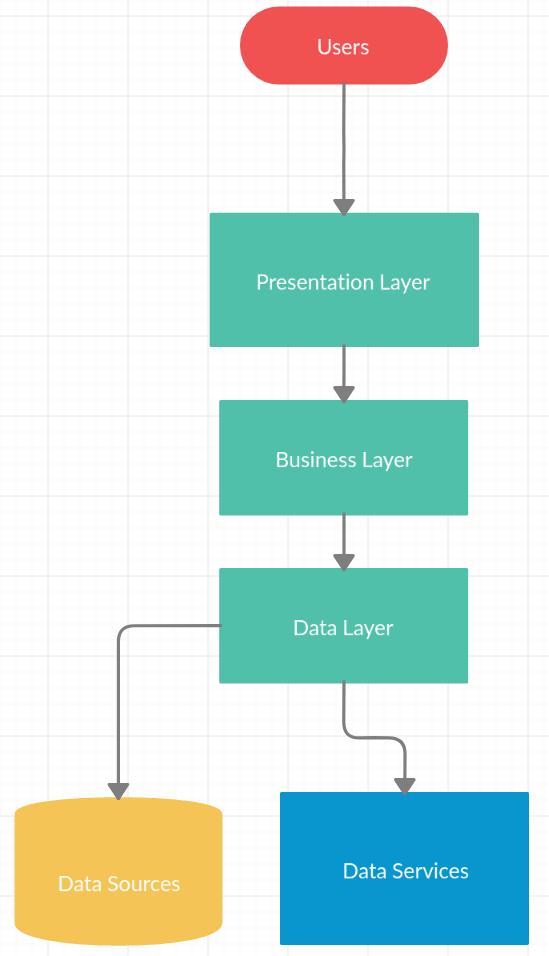
\includegraphics[width=8cm]{DataFlow.png}
\end{center}
By splitting the design and development process into these phases, it allows me to work with modularity - I can develop certain parts of the application without having to deal with problems of dependency or worrying about how they may work with other parts of the application.\\
\\It also means in future, I can update the presentation layer without having effected any of the backend processes, and vice versa - add and develop extra functionality on the backend while leaving the frontend fully functional and intact. After development is finished I can then present the changes to the user.\\

\begin{itemize}
    \item \textbf{Presentation Layer} - Any application (PC/Android/iPhone) that allows the user to access and interface with their data.
    \item \textbf{Business Layer} - An intermediary layer to carry out processing and data coagulation, move processing away from host machines. (API Server, etc.)
    \item \textbf{Data Layer} - A layer that is responsible for storage and provision of data (SQL Server)
    \item \textbf{Data Sources} - The part of the Data Layer that is responsible for storing data (SQL DB)
    \item \textbf{Data Services} - The part of the Business Layer but built into the Data Layer that is responsible for processing of data (Organisation and analysis - SQL Server Services)
\end{itemize}

\begin{table}
\subsection{Project Pipeline}
\centering
\begin{tabular}{|lll|}
\hline
1) Create SQL Database (MySQL DB)                                           &  &  \\
\hline
2) Create User Account (UA) Credentials DB                              &  &  \\
\hline
3) Create User Data DB                                                    &  &  \\
\hline
4) Create Stored Procedures: Create UA, Login, Data Retrieval, Updating, etc. &  &  \\
\hline
5) Hash passwords                                                       &  &  \\
\hline
6) Test DB Stored Procedures - SQL Injection Protection                 &  &  \\
\hline
7) Create RESTful API                                                   &  &  \\
\hline
8) Establish DB Connection from REST API                                &  &  \\
\hline
9) User Account Login over REST                                         &  &  \\
\hline
10) User Account Creation over REST                                      &  &  \\
\hline
11) Data Retrieval over REST                                             &  &  \\
\hline
12) Test REST API - API Key/ Token Access only                           &  &  \\
\hline
13) Basic Test for REST API Procedures                                   &  &  \\
\hline
14) Create WinForm                                                       &  &  \\
\hline
15) Working Log-in WinForm                                               &  &  \\
\hline
16) Working Sign-Up WinForm                                              &  &  \\
\hline
17) Data Representation                                                  &  &  \\
\hline
18) Data Editing/ Presentation                                           &  &  \\
\hline
19) Create WebApp                                                        &  &  \\
\hline
20) Working Log-in WebForm                                               &  &  \\
\hline
21) Working Sign-up WebForm                                              &  &  \\
\hline
22) Data Representation                                                  &  &  \\
\hline
23) Data Editing/ Presentation                                           &  &  \\
\hline
24) Create MobileApp                                                        &  &  \\
\hline
25) Working Log-in MobileForm                                               &  &  \\
\hline
26) Working Sign-up MobileForm                                              &  &  \\
\hline
27) Data Representation                                                  &  &  \\
\hline
28) Data Editing/ Presentation                                           &  &  \\
\hline
29) Finalisation of UI/UX                                                &  &  \\
\hline
30) Create Testing Container (Brute Force Environment)                   &  &  \\
\hline
31) Prepare Datasets                                                     &  &  \\
\hline
32) Bruteforce test REST API                                             &  &  \\
\hline
33) Bruteforce test WinForm                                              &  &  \\
\hline
34) Bruteforce test WebForm                                              &  &  \\
\hline
35) Fix Test Errors + Retest                                             &  &  \\
\hline
36) Prepare Hardcoded test cases                                         &  &  \\
\hline
37) Release to public testing                                            &  &  \\
\hline
38) Start Implementation of ML with Historical Data                      &  &  \\
\hline
39) Contact Advisors for expected output from Data, use data to train AI &  &  \\
\hline
40) Produce future predictions                                           &  &  \\
\hline
\end{tabular}
\end{table}
\newpage

\section{Implementation}
\subsection{Overview}
I will be using an iteration style development where I work through the project pipeline multiple times. I have outlined these are three main phases, Beta, Alpha and Public:\\
\\The \textbf{Beta} Phase is the most basic version of development and the initial phase that I will work on. It focuses on allowing me to become accustomed with the development software I will be using and will allow me to create a more refined version of my Project Pipeline for use in Alpha and Public Phases. Very little thought will be put into the visual aspect of the program, as most work and development will be on algorithmic structure and creating modularity in the system.\\
\\The \textbf{Alpha} Phase will follow the vague structure of the Beta Phase as well as any changes I've made to the Project Pipeline since. I will also start to mock-up some basic visuals for the End User and will begin to take in considerations like privacy and additional features to make my application more enticing.\\
\\The \textbf{Public} Phase may contain modules from the Alpha Phase especially with regards to the backend, a lot more focus will be put on the visual aspect of the application and I will start to develop mobile frameworks as well - since they can use the same back-end as the Desktop Application, I can use my visual mock-ups after translating them to mobile screens.


\subsubsection{Setting up the SQL Server}
I began to familiarise myself with the Microsoft Azure platform, however this was not viable for development as it was costing me almost £60 a month! I then planned to use a SQL Server instance running on my local machine. This would've been fine for local WinForm and WebApp development, however if I was to develop a mobile app or test my applications on other machines, I would not be able to do so. After a few google searches, I found a platform that allowed me to host free MySQL Server instances, Heroku with JawsDB. At release I cannot use this since the free tier plan has many constraints, but it is perfect for development since I will rarely be using more than one connection at a time. Full plan information can be seen in \textbf{\textit{Figure 2 (Appendix)}}.

\subsubsection{A closer look at database structure}
My Database structure is as follows:
\begin{itemize}
    \item \textbf{Database} \textit{pkdb}
    \begin{itemize}
        \item \textbf{Table} \textit{[dbo].prawnkingusers}
        \item \textbf{Table} \textit{[dbo].prawnkingdata}
        \item \textbf{Table} \textit{[dbo].prawnkingusersdatarel}
        \item \textbf{SP} \textit{ADDUSER}
        \item \textbf{SP} \textit{GETID}
        \item \textbf{SP} \textit{MKADMIN}
        \item \textbf{SP} \textit{UINFO}
        \item \textbf{SP} \textit{USEREXISTS}
        \item \textbf{SP} \textit{TACCESS}
        \item \textbf{SP} \textit{ADDTREF}
        \item \textbf{SP} \textit{ADDTANK}
    \end{itemize}
\end{itemize}
I started using Stored Procedures as opposed to sending SQL Queries from the client for multiple reasons:

\begin{itemize}
    \item Protects from Application Cracking - Even if the program becomes cracked or reverse engineered, the functions that can run on the SQL Server are limited as no instructions are passed from the client.
    \item Protects from SQL Server Attacks - Even if the SQL Requests are intercepted, they will not make sense to the intercepter, and even then only functions that already exist on the SQL Server can be run.
\end{itemize}

\subsubsection{Creating the User Accounts table ([dbo].prawnkingusers)}
\textit{Table Creation SQL Query:}
\begin{lstlisting}[language=SQL,
deletekeywords={IDENTITY,INT},
morekeywords={clustered},    
framesep=10pt,
framextopmargin=10pt]
CREATE TABLE `[dbo].prawnkingusers`
(
userID     INT auto_increment,
userName   VARCHAR(50)              NOT NULL,
userPass   VARCHAR(50)              NOT NULL,
FName      VARCHAR(50)              NULL,
LName      VARCHAR(50)              NULL,
PNumber    INT                      NULL,
isAdmin    BIT		            NULL,
CONSTRAINT `[dbo].prawnkingusers_userID_uindex` UNIQUE (userID),
CONSTRAINT `[dbo].prawnkingusers_userName_uindex` UNIQUE (userName),
PRIMARY KEY (userID)
);
\end{lstlisting}

The \textbf{first} field, userID, is created to be a both a Unique Key and a Primary Key. Using a Unique Key means that every user that gets added to the database has their own ID assigned to the. Using a Primary Key means that I can generate non-clustered indexes automatically as a new user is added to the database, simplifying the process, seen by \textit{"auto\_increment"}. I've also defined the field to be non-nullable, meaning that if a user exists, they must have an ID assigned to them. Having unique IDs will help me later on when I start to create relations between tables and user privellege management.\\
\\The \textbf{second} field, userName, is created to be unique, meaning no two users can have the same user name. The username is saved as cleartext.\\
\\The \textbf{third} field, userPass, has no constraints, other than of length 50 characters. The password is saved in a hashed format.\\
\\The \textbf{fourth, fifth and sixth} fields, FName, LName and PNumber, are user information, which will be encrypted using a key.\\
\\The \textbf{last} field, isAdmin, is a boolean containing whether or not the user is an administrator, being an administrator allows the user to carry out tasks with elevated permissions.\\
\\The use for this table is quite self explanatory, it is the table holding data responsible for all User Account Authentication and Privilege management, as well as all personal identifying data for the users.
\subsubsection{Creating the User Data table ([dbo].prawnkingdata)}
\textit{Table Creation SQL Query:}
\begin{lstlisting}[language=SQL,
deletekeywords={IDENTITY,INT},
morekeywords={clustered,LONGETXT},    
framesep=10pt,
framextopmargin=10pt]
CREATE TABLE `[dbo].prawnkingdata`
(
tankID   INT auto_increment,
data     LONGETXT   NULL,
comments LONGETXT   NULL,
CONSTRAINT `[dbo].prawnkingdata_tankID_uindex` unique (tankID),
PRIMARY KEY (tankID)
);
\end{lstlisting}
The \textbf{first} field, tankID, is created to be a both a Unique Key and a Primary Key. Again for the same purposes as userID in the previous table\\
\\The \textbf{second and third} fields, data and comments, will contain the raw data collected from the user as well as any notes, etc that the user decides to save regarding the tank.\\
\\This table is responsible for holding the data of each location in a given user's portfolio, it'll be linked to multiple users in the user accounts table.
\subsubsection{Creating the Relations table ([dbo].prawnkingusersdatarel)}
\textit{Table Creation SQL Query:}
\begin{lstlisting}[language=SQL,
deletekeywords={IDENTITY,INT},
morekeywords={clustered,LONGETXT},    
framesep=10pt,
framextopmargin=10pt]
CREATE TABLE `[dbo].prawnkingusersdatarel`
(
tankID   INT NOT NULL,
userID   INT NOT NULL,
FOREIGN KEY (tankID) REFERENCES `[dbo].prawnkingdata` (TANKID) ON DELETE RESTRICT ON UPDATE CASCADE,
FOREIGN KEY (userID) REFERENCES `[dbo].prawnkingusers` (userID) ON DELETE RESTRICT ON UPDATE CASCADE,
PRIMARY KEY (tankID,userID)
);
\end{lstlisting}
The \textbf{first} field, tankID, is created to be a Foreign Key which references the tankID column from the data table.\\
\\The \textbf{second} field, userID is created to be a Foreign Key which references the UserID column from the user information table.\\
\\This table contains the many-to-many relations between users and different tanks, since many users should be able to access the same tank, and many tanks are usable by the same user.
\subsubsection{Creating the Add User SP (ADDUSER)}
\textit{Stored Procedure Creation SQL Query:}
\begin{lstlisting}[language=SQL,
deletekeywords={IDENTITY,INT},
morekeywords={clustered,OUT, BEGIN, PROCEDURE},    
framesep=10pt,
framextopmargin=10pt]
CREATE PROCEDURE ADDUSER(
IN Usr varchar(50),
IN Pwd varchar(50),
OUT Rtn bit
)

BEGIN
	IF EXISTS(SELECT userID FROM `[dbo].prawnkingusers` WHERE userName = Usr) THEN
		SET Rtn = 0;
	ELSE
		INSERT INTO `[dbo].prawnkingusers` (userName,userPass)
		VALUES(Usr,Pwd);
		SET Rtn = 1;
	END IF;
END;
\end{lstlisting}
This stored procedure adds new user if does not exist given Username and Password. \textbf{Lines 1-5} declare the input parameters (Username and Password to be added) and the output parameter (Rtn, success?)\\
\\\textbf{Lines 8-14} is a conditional statement that checks whether a user with the provided username already exists; If it does, Rtn is set to 0 to signify a failure in account creation. Else, the account details are submitted into the table and a successful Rtn is passed.\\
\\\textit{Stored Procedure Execution SQL Query:}
\begin{lstlisting}[language=SQL,
deletekeywords={IDENTITY,INT},
morekeywords={clustered,OUT, BEGIN, PROCEDURE,CALL},    
framesep=10pt,
framextopmargin=10pt]
--username here
SET @Usr = '';
--password here
SET @Pwd = '';
CALL ADDUSER(
@Usr,
@Pwd,
@Rtn
);
--return here (1 - Success, 0 - Failure)
SELECT @Rt
\end{lstlisting}

\subsubsection{Creating the Get ID SP (GETID)}
\textit{Stored Procedure Creation SQL Query:}
\begin{lstlisting}[language=SQL,
deletekeywords={IDENTITY,INT},
morekeywords={clustered,OUT, BEGIN, PROCEDURE},    
framesep=10pt,
framextopmargin=10pt]
CREATE PROCEDURE GETID( IN Usr VARCHAR(50), IN Pwd VARCHAR(50), OUT Rtn INT )
BEGIN
SET Rtn = (SELECT userID FROM `[dbo].prawnkingusers` WHERE (userPass = Pwd AND userName = Usr));
END
\end{lstlisting}
This stored procedure returns the userID of the user with the provided username and password, given that these are of valid combination. \textbf{Line 1} declares the input parameters (Username and Password to be searched) and the output parameter (Rtn, ID?)\\
\\\textbf{Line 3} Sets the result of the SELECT statement into the Rtn variable. The SELECT statement searches for the provided combination of credentials within the table and returns the respective userID. If no user exists, null is returned.\\
\\\textit{Stored Procedure Execution SQL Query:}
\begin{lstlisting}[language=SQL,
deletekeywords={IDENTITY,INT},
morekeywords={clustered,OUT, BEGIN, PROCEDURE,CALL},    
framesep=10pt,
framextopmargin=10pt]
--username here
SET @Usr = '';
--password here
SET @Pwd = '';
CALL getid(
@Usr,
@Pwd,
@Rtn
);
SELECT @Rtn
--return here (integer - Success, Null - Failure)
\end{lstlisting}

\subsubsection{Creating the User Exists SP (USEREXISTS)}
\textit{Stored Procedure Creation SQL Query:}
\begin{lstlisting}[language=SQL,
deletekeywords={IDENTITY,INT},
morekeywords={clustered,OUT, BEGIN, PROCEDURE},    
framesep=10pt,
framextopmargin=10pt]
CREATE PROCEDURE `USEREXISTS`( IN Usr VarChar(50), OUT Rtn INT )
BEGIN
IF (EXISTS (SELECT userID FROM `[dbo].prawnkingusers` WHERE (userName = Usr))) THEN
SET Rtn = 1;
ELSE
SET Rtn = 0;
END IF;
END
\end{lstlisting}
This stored procedure returns a boolean of whether a username is available for use or not given the username. \textbf{Line 1} declares the input parameters (Username to be searched) and the output parameter (Rtn, Available?)\\
\\\textbf{Line 3} Sets the result of the EXISTS SELECT statement into the Rtn variable. The SELECT statement searches for the provided combination of credentials within the table and returns the respective userID. If no user exists, null is returned. This existance is then converted into a Boolean with the EXISTS statement, this bool is then returned.\\
\\\textit{Stored Procedure Execution SQL Query:}
\begin{lstlisting}[language=SQL,
deletekeywords={IDENTITY,INT},
morekeywords={clustered,OUT, BEGIN, PROCEDURE,CALL},    
framesep=10pt,
framextopmargin=10pt]
--username here
SET @Usr = '';
CALL USEREXISTS(
@Usr,
@Rtn
);
SELECT @Rtn
--return here (1 - Exists, 0 - None)
\end{lstlisting}

\subsubsection{Creating the Make Admin SP (MKADMIN)}
\textit{Stored Procedure Creation SQL Query:}
\begin{lstlisting}[language=SQL,
deletekeywords={IDENTITY,INT},
morekeywords={clustered,OUT, BEGIN, PROCEDURE},    
framesep=10pt,
framextopmargin=10pt]
CREATE PROCEDURE `MKADMIN`(IN Usr varchar(50), IN Pwd varchar(50),IN UsrID int, OUT Rtn bit)
BEGIN
IF EXISTS (SELECT userID FROM `[dbo].prawnkingusers` WHERE userName = Usr AND userPass = Pwd AND `isAdmin?` = 1) THEN
IF EXISTS(SELECT userName FROM `[dbo].prawnkingusers` WHERE userID = UsrID) THEN
UPDATE `[dbo].prawnkingusers`
SET `isAdmin?` = 1
WHERE userID = UsrID;
SET Rtn = 1;
END IF;
ELSE
SET Rtn = 0;
END IF;
END;
\end{lstlisting}
This stored procedure attempts to promote the privelege of a user to admin given another set of user credentials who is already an admin. \textbf{Line 1} declares the input parameters (UserID of user to be promoted, and userName and userPass of the user who is carrying out the promotion) and the output parameter (Rtn, Success?)\\
\\\textbf{Line 3} is  a conditional statement that checks that the admin credentials provided are valid and that the user is actually an admin. If they aren't a failure is returned.\\
\\\textbf{Line 4} is  another conditional statement that checks that a user exists with the userID provided to be able to promote them to admin. Else returns failure.\\
\\\textbf{Lines 5-8} edit the 'isAdmin?' value of the column of the user with the provided userID and sets the return value to 1 - success. This value is then returned.\\
\\\textit{Stored Procedure Execution SQL Query:}
\begin{lstlisting}[language=SQL,
deletekeywords={IDENTITY,INT},
morekeywords={clustered,OUT, BEGIN, PROCEDURE,CALL},    
framesep=10pt,
framextopmargin=10pt]
--username here
SET @Usr = '';
--password here
SET @Pwd = '';
--userID here
SET @UsrID = 0;
CALL mkadmin(
@Usr,
@Pwd,
@UsrID,
@Rtn
);
SELECT @Rtn;
--return here (1 - Exists, 0 - None)
\end{lstlisting}

\subsubsection{Creating the User Info SP (UINFO)}
\textit{Stored Procedure Creation SQL Query:}
\begin{lstlisting}[language=SQL,
deletekeywords={IDENTITY,INT},
morekeywords={clustered,OUT, BEGIN, PROCEDURE},    
framesep=10pt,
framextopmargin=10pt]
CREATE PROCEDURE `uinfo`(IN Usr varchar(50), IN Pwd varchar(50),IN fname varchar(50), IN lname varchar(50), IN pnumber varchar(50), OUT Rtn bit)
BEGIN
IF EXISTS (SELECT userID FROM `[dbo].prawnkingusers` WHERE userName = Usr AND userPass = Pwd) THEN
UPDATE `[dbo].prawnkingusers`
SET `FName` = fname,
`LName` = lname,
`PNumber` = pnumber
WHERE (userName = Usr AND userPass = Pwd);
SET Rtn = 1;
ELSE
SET Rtn = 0;
END IF;
END;
\end{lstlisting}
This stored procedure is used to add optional user information to the database, for future reference, contact, and personalisation options. \textbf{Line 1} declares the input parameters (UseruserName and userPass of the user who is carrying out the data addition, and the corresponding data, and the output parameter (Rtn, Success?)\\
\\\textbf{Line 3} is  a conditional statement that checks that the credentials provided are valid and that the user exists. If they aren't a failure is returned.\\
\\\textbf{Line 4-8} update that given user's information \\
\\\textbf{Line 9} returns a success code.\\
\\\textit{Stored Procedure Execution SQL Query:}
\begin{lstlisting}[language=SQL,
deletekeywords={IDENTITY,INT},
morekeywords={clustered,OUT, BEGIN, PROCEDURE,CALL},    
framesep=10pt,
framextopmargin=10pt]
--username here
set @Usr = '';
--password here
set @Pwd = '';
--first name here
set @fname = '';
--last name here
set @lname = '';
--phone number here
set @pnumber = '';
call uinfo(
@Usr,
@Pwd,
@fname,
@lname,
@pnumber,
@Rtn
);
select @Rtn;
--return here (1 - Exists, 0 - None)
\end{lstlisting}

\subsubsection{Creating the Tank Access SP (UINFO)}
\textit{Stored Procedure Creation SQL Query:}
\begin{lstlisting}[language=SQL,
deletekeywords={IDENTITY,INT},
morekeywords={clustered,OUT, BEGIN, PROCEDURE},    
framesep=10pt,
framextopmargin=10pt]
CREATE PROCEDURE `taccess`(IN UsrID int, OUT rtn varchar(255))
BEGIN
SET rtn =(SELECT GROUP_CONCAT(tankID) FROM `[dbo].prawnkingusersdatarel` WHERE userID=UsrID);
END;
\end{lstlisting}
This stored procedure is used to find the tanks that a user has access to, given the user ID. \textbf{Line 1} declares the input parameters (userID) of the user being queried, and the output parameter (Rtn, Success?)\\
\\\textbf{Line 3} is  a variable set statement that takes the output of the select statement and concatenates it into a single string delimited by commas, and so can be processed as a list of tanks for that user.\\
\\\textit{Stored Procedure Execution SQL Query:}
\begin{lstlisting}[language=SQL,
deletekeywords={IDENTITY,INT},
morekeywords={clustered,OUT, BEGIN, PROCEDURE,CALL},    
framesep=10pt,
framextopmargin=10pt]
--user id here
SET @UsrID = 0;
CALL taccess(
@UsrID,
@Rtn
);
SELECT @Rtn
--return here (Null - No tanks)
\end{lstlisting}


\subsubsection{Creating the Add Tank SP (UINFO)}
\textit{Stored Procedure Creation SQL Query:}
\begin{lstlisting}[language=SQL,
deletekeywords={IDENTITY,INT},
morekeywords={clustered,OUT, BEGIN, PROCEDURE},    
framesep=10pt,
framextopmargin=10pt]
CREATE PROCEDURE `addtank`(IN UsrID int, OUT rtn varchar(255))
BEGIN
IF EXISTS( SELECT userName FROM  `[dbo].prawnkingusers` WHERE userID = UsrID) THEN
INSERT INTO `[dbo].prawnkingdata`(data)
VALUES (null);
INSERT INTO  `[dbo].prawnkingusersdatarel`(tankID, userID) VALUES ((SELECT LAST_INSERT_ID()),UsrID);
SET rtn = 1;
ELSE
SET rtn = 0;
END IF;
END;
\end{lstlisting}
This stored procedure is used to add a new tank to the list of tanks and also create a relationship between the user who created it and that tank. \textbf{Line 1} declares the input parameters (userID) of the user being given a new tank, and the output parameter (Rtn, Success?)\\
\\\textbf{Line 3} is  a conditional statement that checks if the given userID exists in the user accounts db. If it doesn't error (0) is returned.\\
\\\textbf{Lines 4 to 6} run if the conditional statement is successful, it adds a tank to the data db and then adds a relation between the user who created it and the id of the tank that was just created into the relations db.\\
\\\textbf{Line 7} returns the success code.
\\\textit{Stored Procedure Execution SQL Query:}
\begin{lstlisting}[language=SQL,
deletekeywords={IDENTITY,INT},
morekeywords={clustered,OUT, BEGIN, PROCEDURE,CALL},    
framesep=10pt,
framextopmargin=10pt]
--userID here
SET @UsrID = ;
SET @Rtn = '';
CALL addtank(
@UsrID,
@Rtn
);
SELECT @Rtn
--return here (Null - No tanks)
\end{lstlisting}

\subsubsection{Creating the Add Tank Relation SP (UINFO)}
\textit{Stored Procedure Creation SQL Query:}
\begin{lstlisting}[language=SQL,
deletekeywords={IDENTITY,INT},
morekeywords={clustered,OUT, BEGIN, PROCEDURE},    
framesep=10pt,
framextopmargin=10pt]
CREATE PROCEDURE `addtref`(IN UsrID int, IN UsrAddID int, IN tnkID int, OUT rtn varchar(255))
BEGIN
IF EXISTS( SELECT userID FROM  `[dbo].prawnkingusersdatarel` WHERE userID = UsrID and tankID = tnkID ) THEN
INSERT INTO  `[dbo].prawnkingusersdatarel`(tankID, userID) VALUES (tnkID,UsrAddID);
SET rtn = 1;
ELSE
SET rtn = 0;
END IF;
END;
\end{lstlisting}
This stored procedure is used to add a new tank relation between a prexisiting tank and another user. \textbf{Line 1} declares the input parameters (userAddID) of the user being given a new tank, userID of a user already with access to the tank, and the output parameter (Rtn, Success?)\\
\\\textbf{Line 3} is  a conditional statement that checks if the given userID exists in the user accounts db against the provided tankID. If it doesn't error (0) is returned.\\
\\\textbf{Lines 4} adds a new relational record into the relations db with the userID provided in (userAddID) and the tankID\\
\\\textbf{Line 8} returns the success code.
\\\textit{Stored Procedure Execution SQL Query:}
\begin{lstlisting}[language=SQL,
deletekeywords={IDENTITY,INT},
morekeywords={clustered,OUT, BEGIN, PROCEDURE,CALL},    
framesep=10pt,
framextopmargin=10pt]
--userID with access here
set @UsrID = ;
--userID to be given access here
set @UsrAddID = ;
--tankID to be given access to here
set @TankID = 
set @Rtn = '';
call addtref(
@UsrID,
@UsrAddID,
@TankID,
@Rtn
);
SELECT @Rtn
--return here (Null - No tanks)
\end{lstlisting}

\newpage

\section{Bibliography}

\subsection{December 2019:}
\textsuperscript{4}{Ravindra Chikkam - Personal Data Collection Measures}

\subsection{February 2020:}
\textsuperscript{1}{FAO - www.fao.org - "India at a glance"}\\
\textsuperscript{2}{BASF - www.basf.com - "How sustainable farming in India can secure its food for the future"}\\
\textsuperscript{3}{The Fish Site - www.thefishsite.com - "How to Farm Indian White Prawn"}

\section{Appendix}
\subsection{Figures}
\begin{figure}[p]
	\centering
	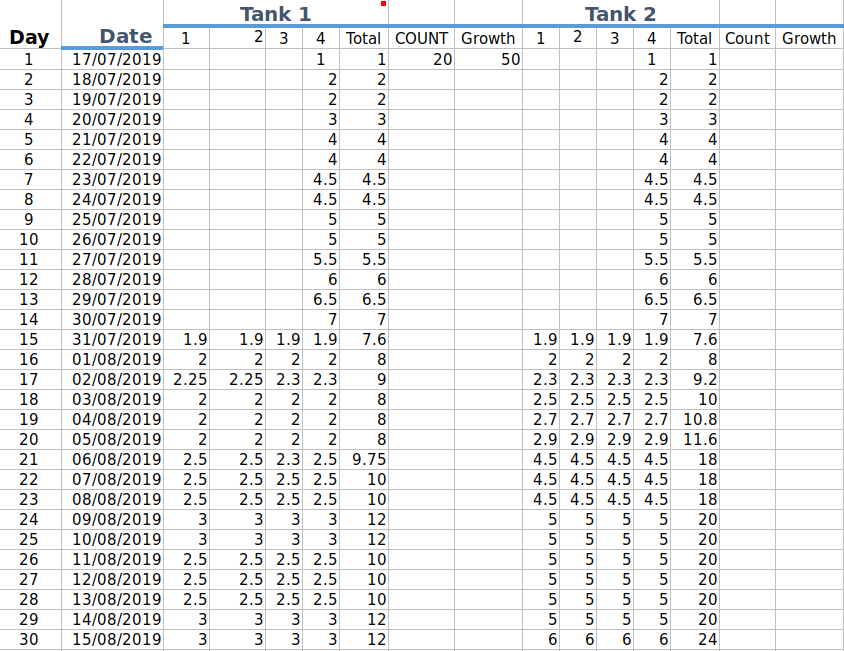
\includegraphics[width=17.2cm]{RaviData.png}
	\caption{\textit{An extract of an eighth of a month's data collected by a small scale aquatics owner.\textsuperscript{[4]}}}
\end{figure}

\begin{figure}[p]
	\centering
	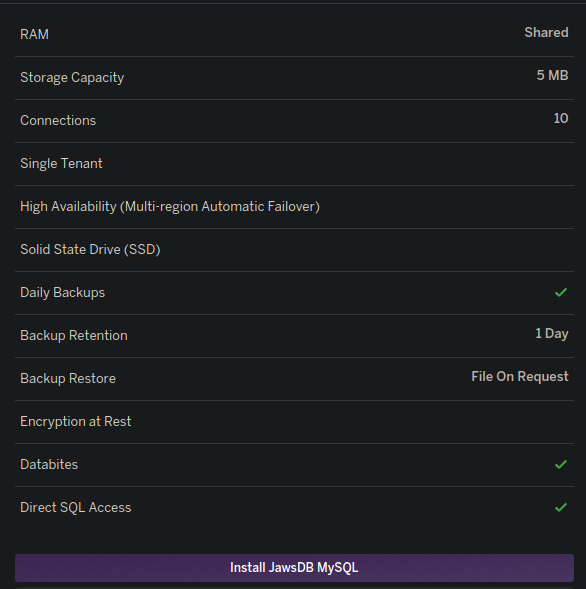
\includegraphics[width=17.2cm]{JawsPlan.png}
	\caption{\textit{The Free Tier Plan from heroku hosting the JawsDB add-on.}}
\end{figure}
\FloatBarrier
\subsection{Source Code}
\end{document}